
\title{Анализ алгоритмов (семинар)}
\author[М. Кузнецов]{Максим Кузнецов}
\institute{ВШЭ, Москва}
\date{16 января 2016}

% Create title page.
\frame{\titlepage} 

%-------------------------------------------------------------------------------

\begin{frame}{Анализ алгоритмов}
  Для некоторого алгоритма с размерами входных данных $\vec{n}$:
  
  \begin{itemize}
    \onslide<+->{
      \item Получить оценку его характеристик, в частности, времени работы $T(\vec{n})$ и количества потребляемой памяти $S(\vec{n})$, в худшем случае [входных данных]
    }
    \onslide<2->{
      \item Рассмотреть лучший и {\em ожидаемый} случаи
    }

    \onslide<3->{
      \item {\em Амортизационный анализ} (усреднение по последовательности операций)
      \item Учёт факторов использования и реализации алгоритма
      \item ...
    }
  \end{itemize}

  \onslide<2>{
    В рамках курса нас чаще всего будет интересовать эти две задачи.
  }
\end{frame}

%-------------------------------------------------------------------------------

\begin{frame}{Асимптотические классы $\Omega$/$\Theta$/$O$}

  $$
    \begin{aligned}
    f(n) \in O(g(n)): &~ \exists c_1 ~~ \exists n_0 ~~ \forall n > n_0 ~\to~ f(n) \leqslant c_1 \cdot g(n) \\
    f(n) \in \Omega(g(n)): &~ \exists c_2>0 ~~ \exists n_0 ~~ \forall n > n_0 ~\to~ f(n) \geqslant c_2 \cdot g(n) \\
    f(n) \in \Theta(g(n)): &~ f(n) \in O(g(n)) ~~\&~~ f(n) \in \Omega(g(n))
    \end{aligned}
  $$

  \begin{figure}
    \centering
    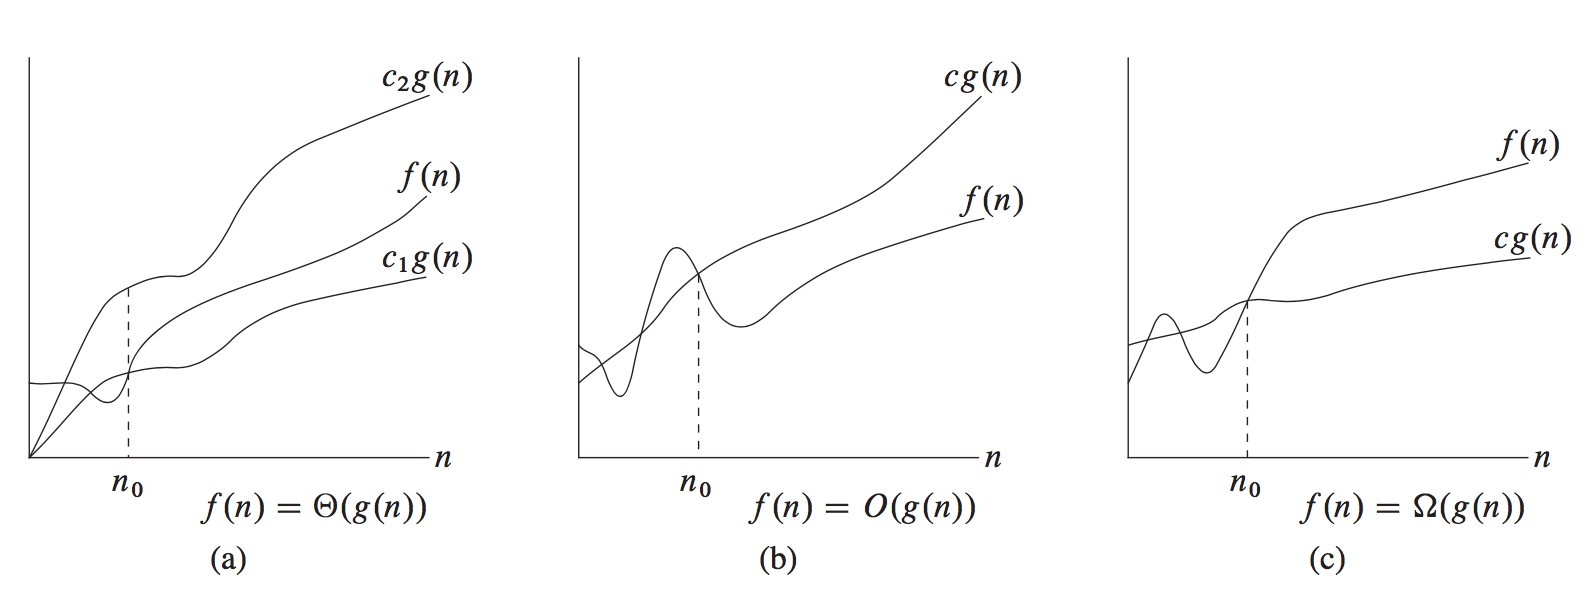
\includegraphics[width=11.5cm]{classes.png}
  \end{figure}

\end{frame}

%-------------------------------------------------------------------------------

\begin{frame}{Использование в информатике}

\onslide<+->{
  Формальное определение позволяет написать $n^2 \in O(n^3)$ или $n^2 \in \Omega(n)$,
  что даёт мало информации с точки зрения анализа алгоритмов.
}

\onslide<+->{
  Интересны следующие три случая:
  $$
  \begin{gathered}
    \lim_{n\to\infty} \frac{f(n)}{g(n)} = \\~~~
    \begin{cases}
    0         &  \Rightarrow ~  f(n) \prec g(n) ~  \text{($f$ растёт медленнее чем $g$)} \\
    \infty    &  \Rightarrow ~  f(n) \succ g(n) ~  \text{($f$ растёт быстрее чем $g$)} \\
    < \infty  &  \Rightarrow ~  f(n) \asymp g(n) ~  \text{($f$ и $g$ растут одинаково)} \\
    \end{cases}
  \end{gathered}
  $$
}

\onslide<+->{
  Третий случай соответствует <<точной>> оценке роста $f(n) \in \Theta(g(n))$. {\bf Однако,
  в информатике (и наших занятиях в дальнейшем) для одинаково растущих функций
  применяют обозначение $f(n) = O(g(n))$}.
}

\end{frame}


%-------------------------------------------------------------------------------

\begin{frame}{Часто встречающиеся классы функций}%
\begin{itemize}
  \item {\em Константы}, $f(n)=1$
   \item {\em Логарифмические}, $f(n)=\lg(n)$
   \item {\em Линейные}, $f(n)=n$
   \item {\em Линейно-логарифмические}, $f(n)=n\lg(n)$
   \item {\em Квадратичные}, $f(n)=n^2$
   \item {\em Кубические}, $f(n)=n^3$
   \item {\em Экспоненциальные}, $f(n)=c^n$ где $c=\const$
   \item {\em Факториальные}, $f(n)=n!$
\end{itemize}%
$$
\boxed{
  1 ~~\prec~~ \lg(n) ~~\prec~~ n ~~\prec~~ n\lg(n) ~~\prec~~ n^2 ~~\prec~~ n^3 ~~\prec~~ c^n ~~\prec~~ n!
}
$$
%
\onslide<+->{
Формула Стирлинга:
$$
n! \sim \sqrt{2\pi n} \left(\frac{n}{e}\right)^n
$$
}

\end{frame}


%-------------------------------------------------------------------------------

\begin{frame}{Часто встречающиеся классы функций}

  \begin{figure}
    \centering
    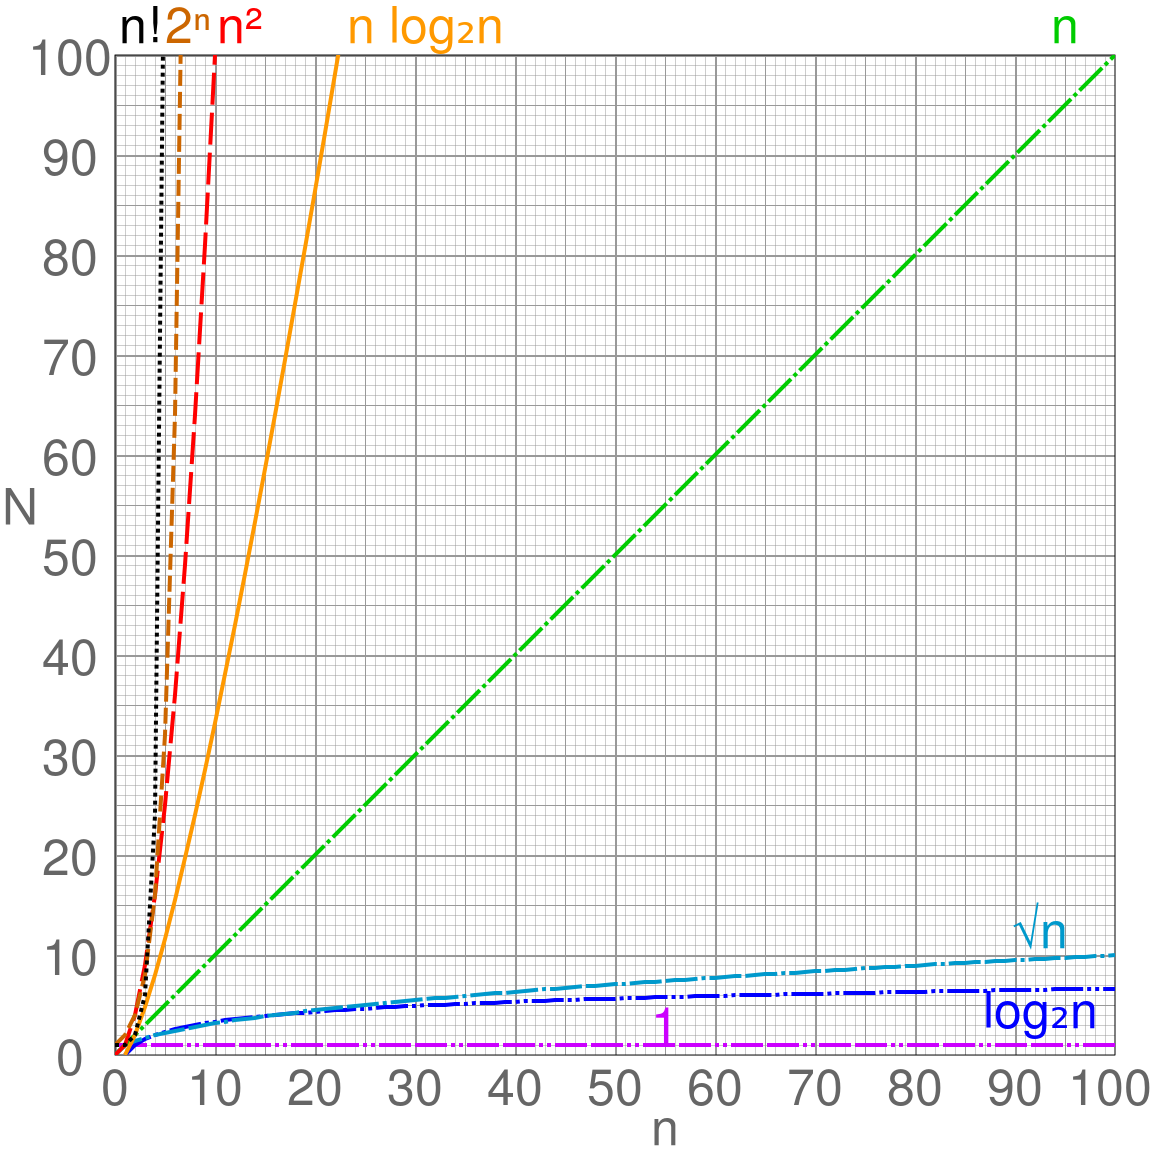
\includegraphics[width=8cm]{funcs.png}
  \end{figure}

\end{frame}

%-------------------------------------------------------------------------------

\begin{frame}[fragile]{Быстрое возведение в степень}

Input: $a$, $b$ ~~~~~ Output: $a^b$

Воспользуемся двоичным разложением $b$:
$$
\begin{gathered}
b = \sum_{i} 2^i \cdot c_i ,~~~ c_i = \{0, 1\} \\
a^b = a^{\sum_{i} 2^i \cdot c_i} = \prod_{i: c_i \neq 0} \cdot a^{2^i}
\end{gathered}
$$

\begin{verbatim}
def pow(a, b):
    r, m = 1, a                      # O(1)
    while b:  
        if b % 2: r *= m             # O(1)
        b = b // 2                   # O(1)
        m = m * m                    # O(1)
    return r
\end{verbatim}

\onslide<2>{
  $$
  \boxed{T(b) = O(\lg(b))}
  $$
}

\end{frame}

%-------------------------------------------------------------------------------

\begin{frame}[fragile]{Числа Фибоначчи}

$$
F_n = \begin{cases}
0 & n = 0\\
1 & n = 1\\
F_{n-1} + F_{n-2} & n > 1
\end{cases}
$$

$$
0, 1, 1, 2, 3, 5, 8, 13, 21, 34, 55, 89, 144, ...
$$

\begin{verbatim}
def fib(n):
  if n == 0: return 0
  elif n == 1: return 1
  return fib(n-1) + fib(n-2)
\end{verbatim}

\onslide<+->{
  $$
  T(n) = 3 + T(n-1) + T(n-2) > F(n)
  $$
}
\onslide<+->{
  $$
  \begin{gathered}
  \lim_{n \to \infty} F_{n+1}/F_n = (1 + \sqrt{5})/2 \approx 1.618 \\
  F_n > (1.6)^n ~~~\Rightarrow~~~ \boxed{T(n) = O(c^n)}
  \end{gathered}
  $$
}
\end{frame}

%-------------------------------------------------------------------------------

\begin{frame}[fragile]{Умножение Карацубы}

Input: $x$, $y$ ~~~~~ Output: $x \cdot y$

Работаем в десятичной системе: пусть $x$ и $y$ содержат по $n$ цифр. Выберем $m<n$, например $m = \lceil n/2 \rceil$:%
%
$$
\begin{gathered}
x = x_1 \cdot 10^m + x_0\\
y = y_1 \cdot 10^m + y_0
\end{gathered}
$$%
%%
$$
xy = (x_1 \cdot 10^m + x_0)(y_1 \cdot 10^m + y_0)
     \equiv z_2 \cdot 10^{2m} + z_1 \cdot 10^{m} + z_0
$$%
%
где%
$$
\begin{gathered}
z_0 = x_0 y_0   ~~~~~~~~~~  z_2 = x_1 y_1\\
z_1 = x_1 y_0 + x_0 y_1\\
\end{gathered}
$$%
или, эквивалентно:
$$
z_1 = (x_1 + x_0)(y_1 + y_0) - z_2 - z_0
$$

\onslide<2>{
  $$
  \boxed{
    T(n) = 3T(\lceil n/2 \rceil) + cn + d = \Theta(n^{\log_{2} 3})
  }
  $$
}

\end{frame}

%-------------------------------------------------------------------------------


\begin{frame}{Литература}

\begin{itemize}
  \item {\em Algorithm Design Manual} by Steven Skiena (2nd edition)
   \item {\em Introduction to Algorithms} by Cormen et al
\end{itemize}%

\end{frame}

%-------------------------------------------------------------------------------
